\subsection{Benchmarks}
\label{subsec:exp2}
In this section, we present the results obtained through the experiments on some optimization aspects of generated code. 
Specifically, two questions related to memory consumption and runtime performance of generated code are posed. 

\noindent
\tb{\ti{Research question 2:}} \ti{Runtime performance and memory usage is undoubtedly critical in real-time and embedded systems. Particularly, in event-driven systems, the performance is measured by event processing speed. Does code generated by the presented approach outperform existing approaches and use less memory?}



\noindent
\tb{Experimental dataset:} Two state machine examples are obtained by the preferred benchmark used by the Boost C++ libraries \cite{boost} in \cite{benchmark}. One simple example \cite{simpleexample} only consists of atomic states and another \cite{compositeexample} both atomic and composite states. 
Tools such as Sinelabore (which efficiently generates code from UML State Machines created by various modeling tools such as Magic Draw \cite{Magicdraw}, Enterprise Architect \cite{EA}) and QM \cite{QM}, which generate code from state machines, and C++ libraries (Boost Statechart \cite{Statechart}, Meta State Machine (MSM) \cite{MSM}, C++ 14 MSM-Lite \cite{benchmark}, and functional programming like-EUML\cite{EUML}) are used for evaluation. 
%The tools are Sinelabore, which efficiently generates code from UML State Machines created by various modeling tools such as Magic Draw \cite{Magicdraw}, Enterprise Architect \cite{EA}, and QM \cite{QM}. 
%C++ libraries are Boost Statechart \cite{Statechart}, Meta State Machine (MSM) \cite{MSM}, MSM-Lite \cite{MSMLite}, and EUML \cite{euml}.

\noindent
\tb{Experimental procedures:} We use a Ubuntu virtual machine 64 bit (RAM, memory, Ghz??) hosted by a Windows 7 machine. 
For each tool and library, we created two applications corresponding to the two examples, generated C++ code and compiled it two modes: normal (N), by default GCC compiler, and optimal (O) with options -O2 -s. 
11 millions of events are generated and processed by the simple example and more than 4 millions for the composite example. 
%More than 4 millions of events are processed by the composite example. 
Processing time is measured for each case. 

\subsubsection{Speed} ~\\
\noindent
\tb{Results:} Table \ref{table-speed} shows the median of event processing time. 
In the normal compilation mode (N), Boost Statechart, MSM, MSMLite, EUML are quite slow. 
Only Sinelabore and QM are performantly comparable with our approach. 
The table also shows that the optimization of GCC is significant. 
MSM and MSMLite run faster than Sinelabore and QM.   
Fig. \ref{fig:boxplot} compares the performance of these approaches to that of our approach.
%Boxplots in Fig. \ref{fig:boxplotsimple} and \ref{fig:boxplotcomposite} compare the performance of these approaches to that of our approach for the two examples, respectively. 
%In both of the simple and composite examples, 
Our approach processes faster around 40 milliseconds than the fastest approach within the scope of the experiment.
It is seen that, even without GCC optimizations, code generated by our approach significantly runs faster than that of EUML and QM with the optimizations. 
When compiled with the optimizations, our approach improves the event processing speed. 
Even, in case of composite, our approach does not produce any slowness compared to the simple example. 


% Please add the following required packages to your document preamble:
% \usepackage{multirow}
\begin{comment}
\begin{table*}[]
	\centering
	\caption{Event processing speed in ms}
\label{my-label}
\begin{tabular}{|l|l|l|l|l|l|l|l|l|l|l|l|l|l|l|l|l|}
	\hline
	\multicolumn{1}{|c|}{\multirow{2}{*}{Test}} & \multicolumn{2}{c|}{SC} & \multicolumn{2}{c|}{MSM} & \multicolumn{2}{c|}{MSM-Lite} & \multicolumn{2}{c|}{EUML} & \multicolumn{2}{c|}{Sinelabore} & \multicolumn{2}{c|}{QM} & \multicolumn{2}{l|}{Umple} & \multicolumn{2}{c|}{Our approach} \\ \cline{2-17} 
	\multicolumn{1}{|c|}{}                      & N           & O         & N            & O         & N              & O            & N            & O          & N               & O             & N          & O          & N            & O           & N                & O              \\ \hline
	Simple                                      & 13705,75    & 1658,1    & 5249,57      & 70,63     & 833,67         & 79,37        & 10867,93     & 109,97     & 141,03          & 79,93         & 285,9      & 229,27     & X            & X           & 106,87           & 25,37          \\ \hline
	Composite                                   & 5353,03     & 820,63    & 3546,1       & 46,73     & 516,87         & 65,17        & 4225,57      & 92,3       & 100,03          & 86,03         & 146,23     & 97,57      & X            & X           & 36,47            & 1,40           \\ \hline
\end{tabular}
\end{table*}
\end{comment}

\begin{comment}
\begin{table*}[]
	\centering
	\caption{Event processing speed in ms}
	\label{table-speed}
	\begin{tabular}{|l|l|l|l|l|l|l|l|l|l|l|l|l|l|l|l|l|}
		\hline
		\multicolumn{1}{|c|}{\multirow{2}{*}{Test}} & \multicolumn{2}{c|}{SC} & \multicolumn{2}{c|}{MSM} & \multicolumn{2}{c|}{MSM-Lite} & \multicolumn{2}{c|}{EUML} & \multicolumn{2}{c|}{Sinelabore} & \multicolumn{2}{c|}{QM} & \multicolumn{2}{l|}{Umple} & \multicolumn{2}{c|}{Our approach} \\ \cline{2-17} 
		\multicolumn{1}{|c|}{}                      & N           & O         & N            & O         & N              & O            & N            & O          & N               & O             & N          & O          & N            & O           & N                & O              \\ \hline
		Simple                                      & 13706    & 1658    & 5250      & 71     & 834         & 79        & 10868     & 110     & 141          & 80         & 286      & 229     & X            & X           & 107           & 25,4          \\ \hline
		Composite                                   & 5353     & 821    & 3546       & 47     & 517         & 65        & 4225,6      & 92       & 100          & 86         & 146     & 98      & X            & X           & 36,5            & 1,40           \\ \hline
	\end{tabular}
\end{table*}
\end{comment}

\begin{table*}[]
	\centering
	\caption{Event processing speed in ms}
	\label{table-speed}
	\begin{tabular}{|l|l|l|l|l|l|l|l|l|l|l|l|l|l|l|}
		\hline
		\multicolumn{1}{|c|}{\multirow{2}{*}{Test}} & \multicolumn{2}{c|}{SC} & \multicolumn{2}{c|}{MSM} & \multicolumn{2}{c|}{MSM-Lite} & \multicolumn{2}{c|}{EUML} & \multicolumn{2}{c|}{Sinelabore} & \multicolumn{2}{c|}{QM} & \multicolumn{2}{c|}{PSM} \\ \cline{2-15} 
		\multicolumn{1}{|c|}{}                      & N           & O         & N            & O         & N              & O            & N             & O         & N               & O             & N          & O          & N           & O          \\ \hline
		Simple                                      & 13706       & 1658      & 5250         & 71        & 834            & 79           & 10868         & 110       & 141             & 80            & 286        & 229        & 107         & 25,4       \\ \hline
		Composite                                   & 5353        & 821       & 3546         & 47        & 517            & 65           & 4225,6        & 92        & 100             & 86            & 146        & 98         & 36,5        & 1,40       \\ \hline
	\end{tabular}
\end{table*}

\begin{figure}
	\centering
	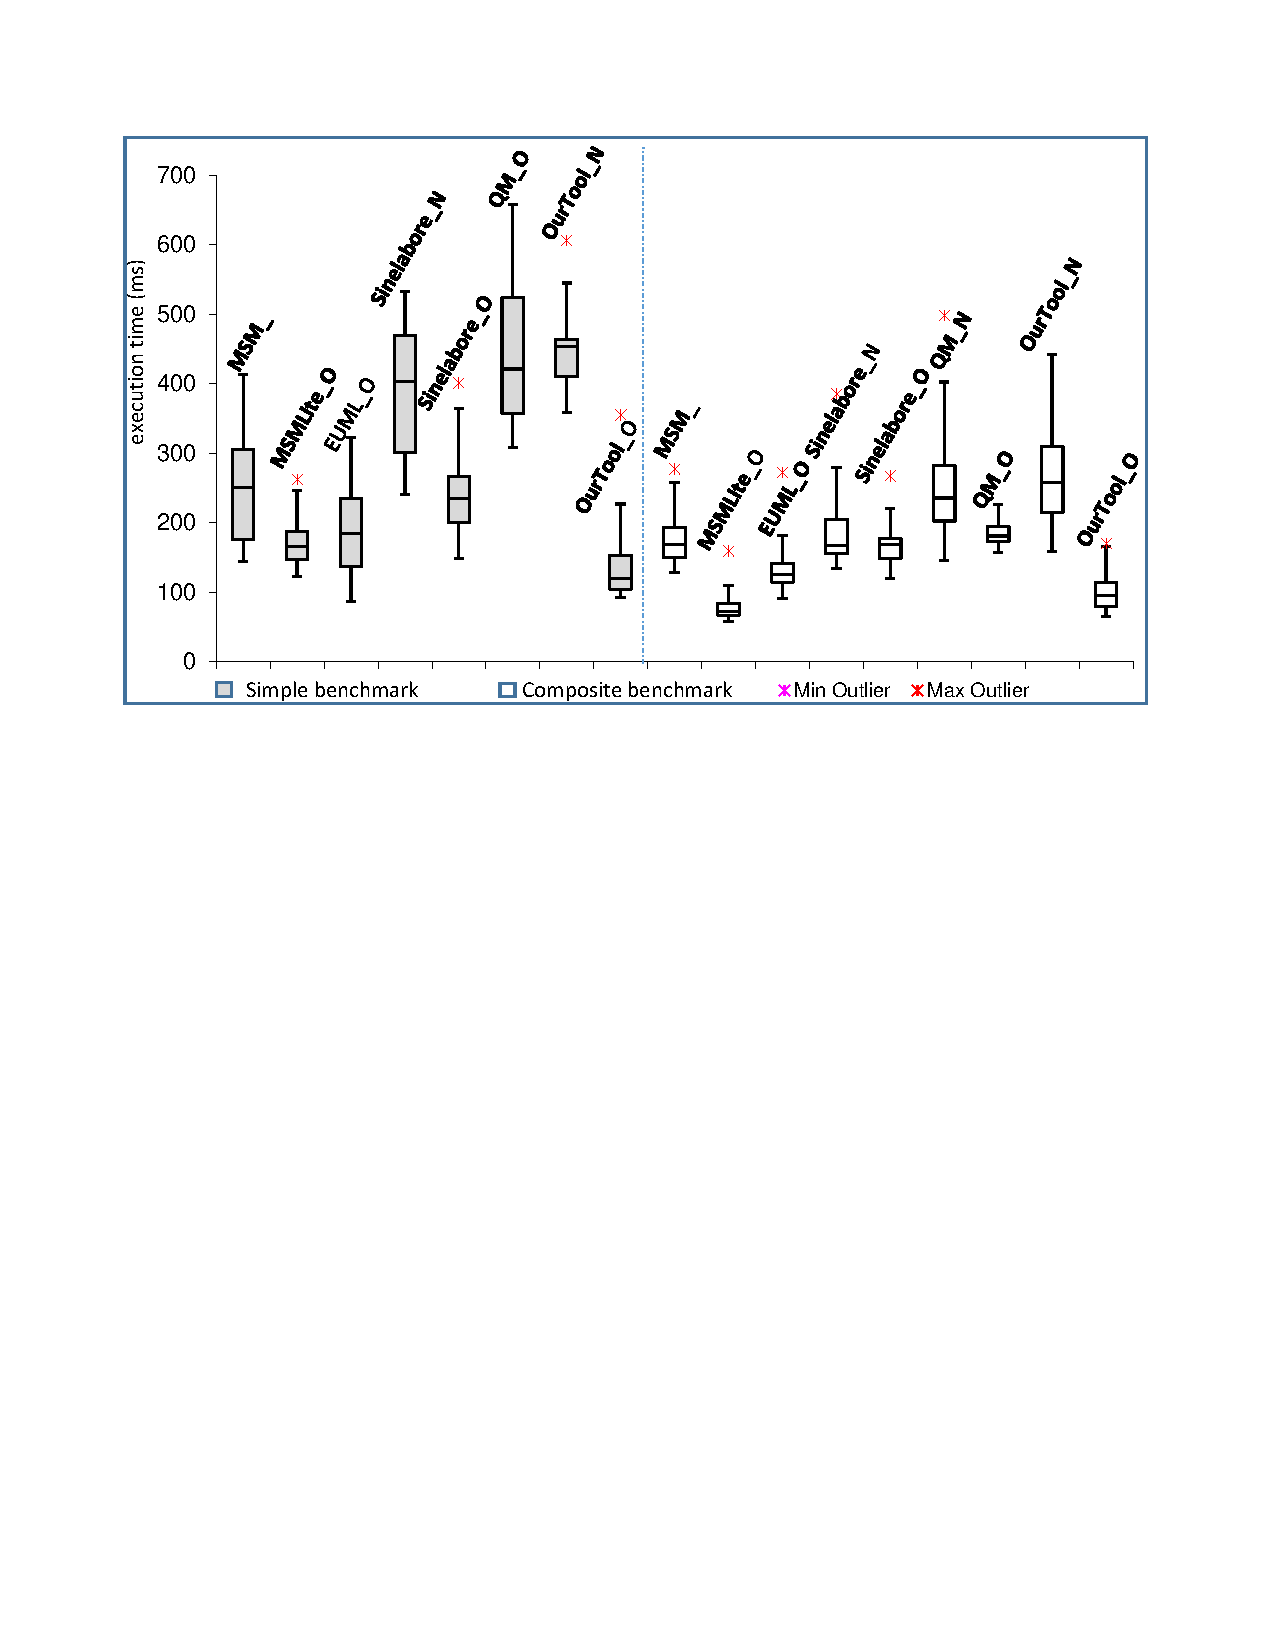
\includegraphics[clip, trim=2.8cm 18.0cm 1.7cm 2.5cm, width=\columnwidth]{experiments/box-plot-mine.pdf}
	\caption{Event processing speed for the benchmark} 
	\label{fig:boxplot}
\end{figure}

\begin{comment}
\begin{figure}
	\centering
	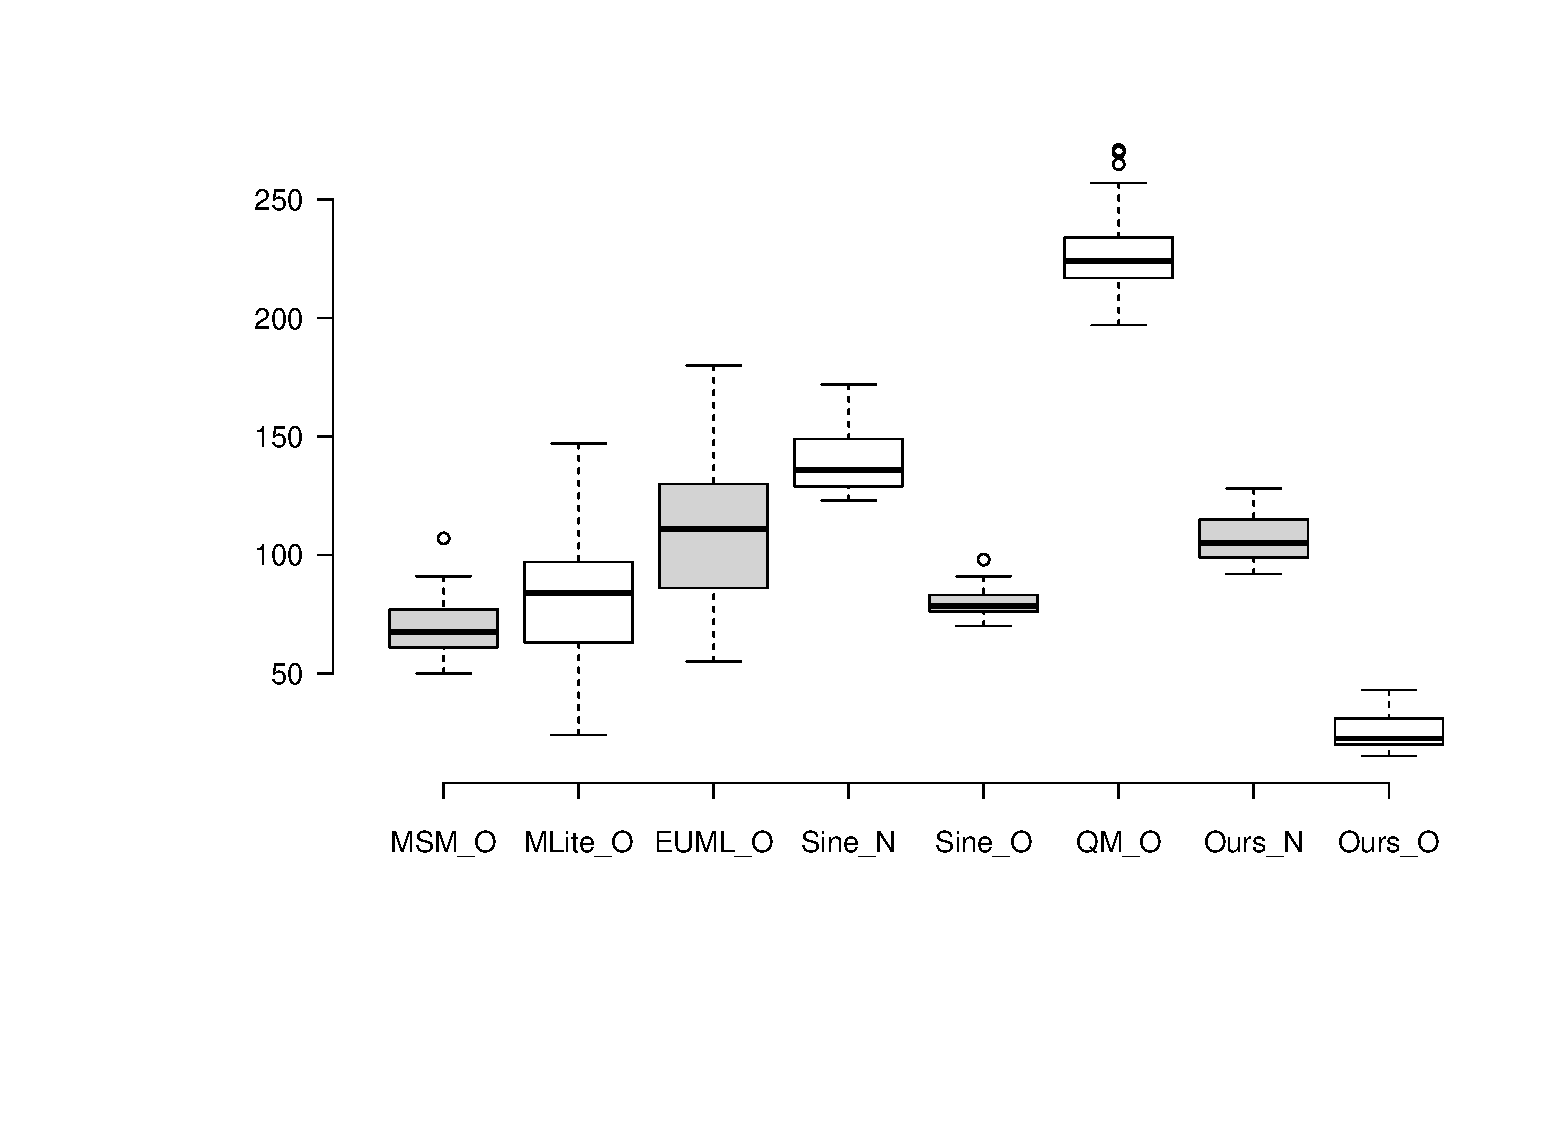
\includegraphics[clip, trim=4.2cm 4.6cm 1.7cm 2.3cm, width=\columnwidth]{figures/boxplotsimple.pdf}
	\caption{Event processing speed for the \ti{Simple} benchmark} 
	\label{fig:boxplotsimple}
\end{figure}

\begin{figure}
	\centering
	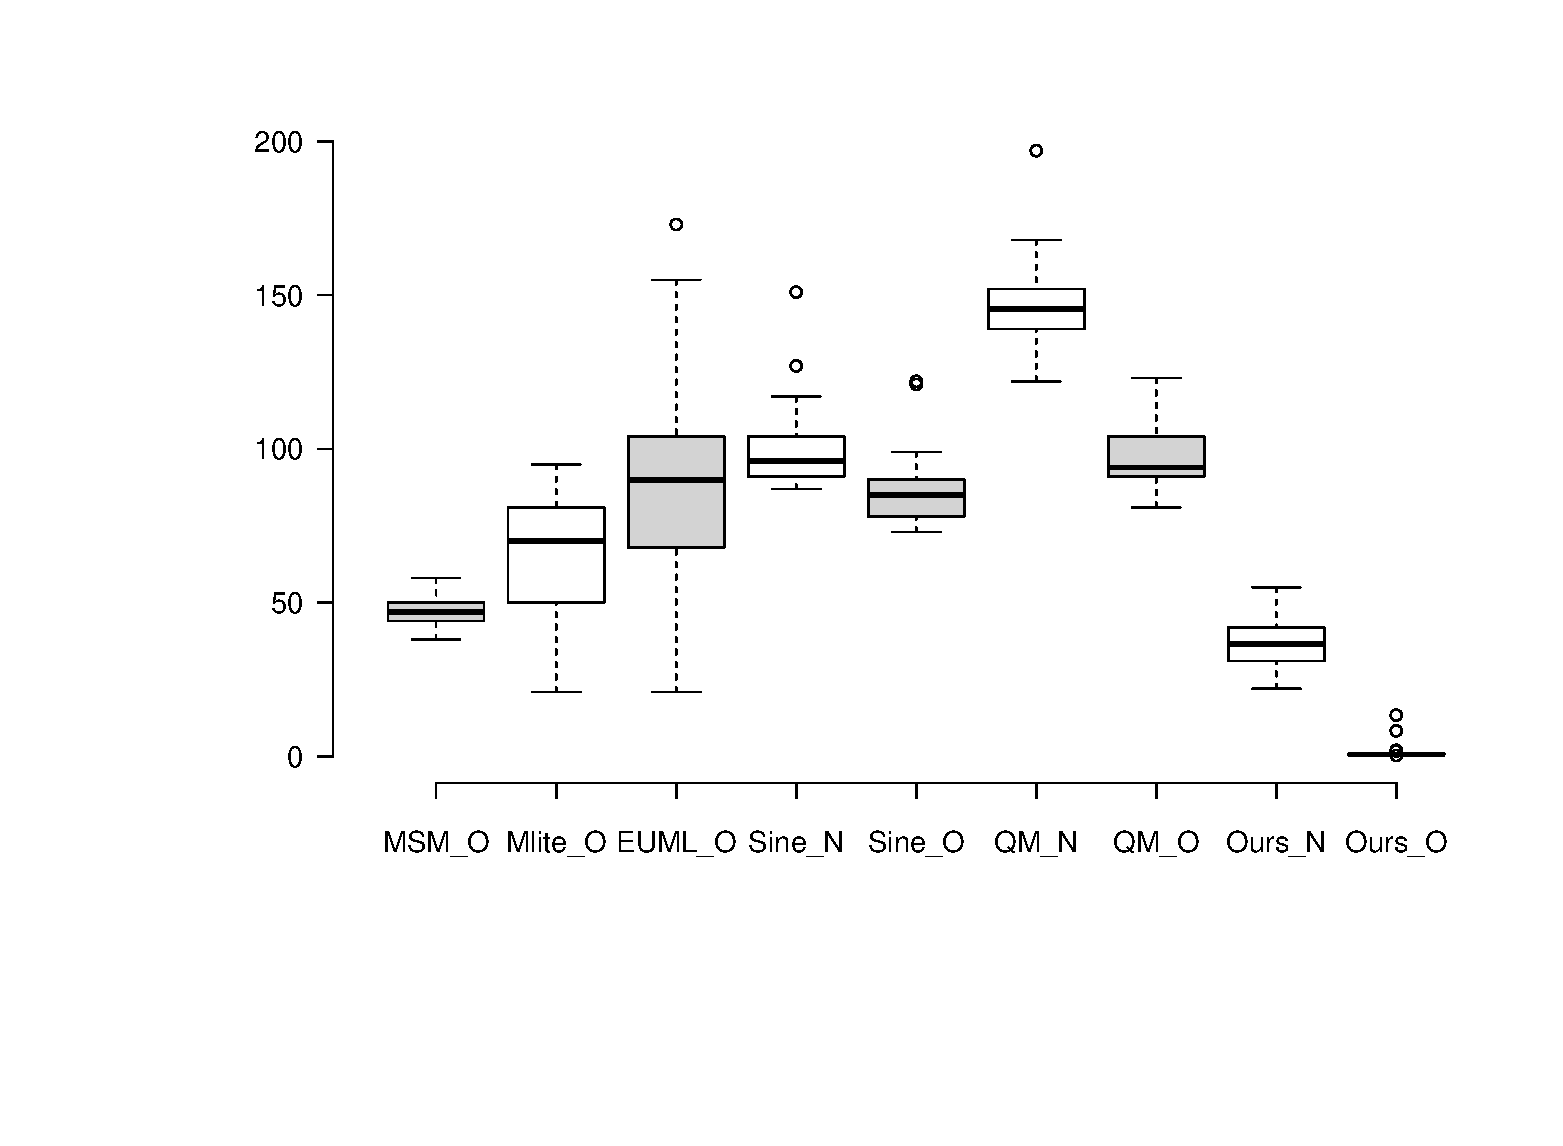
\includegraphics[clip, trim=4.2cm 4.6cm 1.7cm 1.8cm, width=\columnwidth]{figures/boxplotcomposite.pdf}
	\caption{Event processing speed for the \ti{Composite} benchmark} 
	\label{fig:boxplotcomposite}
\end{figure}
\end{comment}


\subsubsection{Binary size and runtime memory consumption} ~\\
\noindent
\tb{Result:} Table \ref{table-size} shows the executable size for the examples compiled in two modes.
It is seen that, in GCC normal mode, Sinelabore generates the smallest executable size while our approach takes the second place.
When using the GCC optimization options, QM and our approach require less static memory than others. 

Considering runtime memory consumption, we use the Valgrind Massif profiler\cite{Massif} to measure memory usage. 
Table \ref{table:usage} shows the measurements for the composite example. 
Compared to others, code generated by our approach requires a slight overhead runtime memory usage (1KB).
This is predictable since the major part of the overhead is used for C++ multi-threading using POSIX Threads and resource control using POSIX Mutex and Condition. 
However, the overhead is small and acceptable (1KB). 


\begin{comment}
\begin{table*}[]
	\centering
	\caption{Executable size in Kb}
	\label{table-size}
	\begin{tabular}{|l|l|l|l|l|l|l|l|l|l|l|l|l|l|l|l|l|}
		\hline
		\multirow{2}{*}{Test} & \multicolumn{2}{c|}{SC} & \multicolumn{2}{c|}{MSM} & \multicolumn{2}{c|}{MSM-Lite} & \multicolumn{2}{c|}{EUML} & \multicolumn{2}{c|}{Sinelabore} & \multicolumn{2}{c|}{QM} & \multicolumn{2}{l|}{Umple} & \multicolumn{2}{c|}{Our approach} \\ \cline{2-17} 
		& N           & O         & N           & O          & N              & O            & N            & O          & N              & O              & N          & O          & N            & O           & N               & O               \\ \hline
		Simple                & 320      & 63,9     & 414,6      & 22,9      & 107,3         & 10,6        & 2339      & 67,9      & 16,5          & 10,6          & 22,6      & 10,5      &       X       &       X      & 21,5           & 10,6           \\ \hline
		Composite             & 435,8      & 84,4     & 837,4      & 31,1      & 159,2         & 10,9        & 4304,8      & 92,5      & 16,6          & 10,6          & 23,4      & 21,5      & X           & X          & 21,6           & 10,6           \\ \hline
	\end{tabular}
\end{table*}
\end{comment}

\begin{table*}[]
	\centering
	\caption{Executable size in Kb}
	\label{table-size}
	\begin{tabular}{|l|l|l|l|l|l|l|l|l|l|l|l|l|l|l|}
		\hline
		\multirow{2}{*}{Test} & \multicolumn{2}{c|}{SC} & \multicolumn{2}{c|}{MSM} & \multicolumn{2}{c|}{MSM-Lite} & \multicolumn{2}{c|}{EUML} & \multicolumn{2}{c|}{Sinelabore} & \multicolumn{2}{c|}{QM} & \multicolumn{2}{c|}{PSM} \\ \cline{2-15} 
		& N           & O         & N           & O          & N              & O            & N            & O          & N              & O              & N          & O          & N           & O          \\ \hline
		Simple                & 320         & 63,9      & 414,6       & 22,9       & 107,3          & 10,6         & 2339         & 67,9       & 16,5           & 10,6           & 22,6       & 10,5       & 21,5        & 10,6       \\ \hline
		Composite             & 435,8       & 84,4      & 837,4       & 31,1       & 159,2          & 10,9         & 4304,8       & 92,5       & 16,6           & 10,6           & 23,4       & 21,5       & 21,6        & 10,6       \\ \hline
	\end{tabular}
\end{table*}

%\subsubsection{Runtime memory consumption}

\begin{table}[]
	\centering
	\caption{Runtime memory consumption in KB. Columns (1) to (7) are SC, MSM, MSM-Lite, EUML, Sinelabore, QM, and our approach, respectively.}
	\label{table:usage}
	\begin{tabular}{|l|l|l|l|l|l|l|l|l|}
		\hline
		Test      & (1)    & (2)  & (3) & (4) & \begin{tabular}[c]{@{}l@{}}(5)\end{tabular} & (6)    & \begin{tabular}[c]{@{}l@{}}(7)\end{tabular} \\ \hline
		Composite & 76.03 & 75.5 & 75.8  & 75.5 & 75.8                                                  & 75.7      & 76.5                                                   \\ \hline
	\end{tabular}
\end{table}